%ju 17-Sep-22 01-Grundlagen-Elektrotechnik.tex
\newpage

\section{Spannung}\label{spannung}

Spannung ist das Ausgleichsbestreben der Elektronen von negativem Pol
zum positiven Pol.

\textbf{Spannung} $U \quad \text{[Volt]} \quad [V]$

\emph{italienischer Physiker Alessandro Volta (1745-1827)}

\begin{table}[!ht]% hier: !ht 
\centering 
	\caption{}% \label{tab:}%% anpassen 
\begin{tabular}{@{}llll@{}}
\hline
\textbf{Einheit} & \textbf{Abk.} & \textbf{Zahl} &
\textbf{Exponentialschreibweise} \\
\hline
kilo V & $[KV]$ & $1000~V$ & $\num{1,0e3}~V$ \\
Volt & $[V]$ & $1~V$ & $\num{1,0e0}~V$ \\
milli V & $[mV]$ & $0,001~V$ & $\num{1,0e-3}~V$ \\
\hline
\end{tabular} 
\end{table}

\section{Widerstand}\label{widerstand}

Widerstand ist das Hemmen der Fortbewegung durch die Atome des
Leiterwerkstoffes, auf die die Elektronen treffen, um sich durch den
Leiter zu bewegen.

\textbf{Widerstand} $R \quad \text{[Ohm]} \quad [\Omega]$

\emph{deutsche Physiker Georg Simon Ohm (1789-1854)}

resistor = Widerstand

\begin{table}[!ht]% hier: !ht 
\centering 
	\caption{}% \label{tab:}%% anpassen 
\begin{tabular}{@{}llll@{}}
\hline
\textbf{Einheit} & \textbf{Abk.} & \textbf{Zahl} &
\textbf{Exponentialschreibweise} \\
\hline
Mega $\Omega$ & $[M\Omega]$ & $1000000~\Omega$ &
$\num{1,0e6}~\Omega$ \\
Kilo $\Omega$ & $[K\Omega]$ & $1000~\Omega$ &
$\num{1,0e3}~\Omega$ \\
Ohm & $[\Omega]$ & $1~\Omega$ & $\num{1,0e0}~\Omega$ \\
milli $\Omega$ & $[m\Omega]$ & $0,001~\Omega$ &
$\num{1,0e-3}~\Omega$ \\
\hline
\end{tabular} 
\end{table}

\newpage

\section{Strom}\label{strom}

Strom ist die gerichtete Bewegung der Elektronen. Ursache für den
Stromfluss ist die Spannung.

\textbf{Strom} $I \quad \text{[Ampere]} \quad [A]$

\emph{französischer Physiker André-Marie Ampère (1775-1836)}

I = Intensität, International >>Ampere<<

\begin{table}[!ht]% hier: !ht 
\centering 
	\caption{}% \label{tab:}%% anpassen 
\begin{tabular}{@{}llll@{}}
\hline
\textbf{Einheit} & \textbf{Abk.} & \textbf{Zahl} &
\textbf{Exponentialschreibweise} \\
\hline
kilo A & $[KA]$ & $1000~A$ & $\num{1,0e3}~A$ \\
Ampere & $[A]$ & $1~A$ & $\num{1,0e0}~A$ \\
milli A & $[mA]$ & $0,001~A$ & $\num{1,0e-3}~A$ \\
micro A & $[\mu A]$ & $0,000001~A$ & $\num{1,0e-6}~A$ \\
nano A & $[nA]$ & $0,000000001~A$ & $\num{1,0e-9}~A$ \\
\hline
\end{tabular} 
\end{table}

\textbf{Stromflussrichtungen}

\begin{figure}[!ht]% hier: !ht
\centering
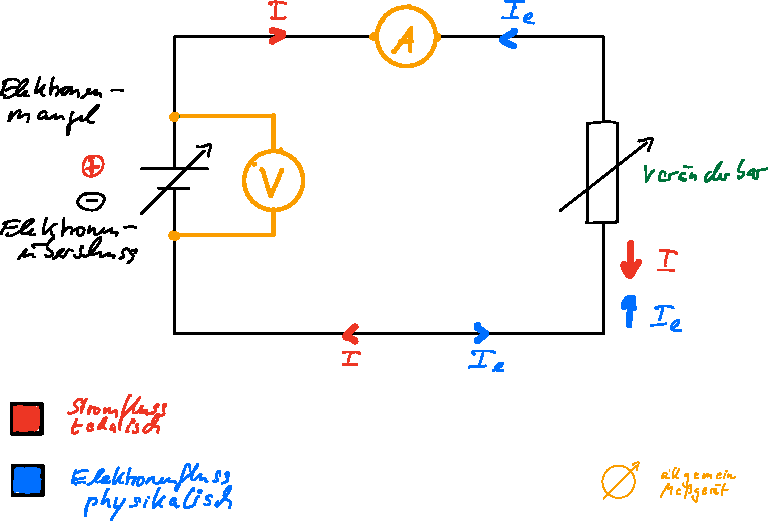
\includegraphics[width=0.6\textwidth]{images/Skizze/06_Stromfluss_Messen_Skizze.pdf}
\caption{Stromfluss und Messen}
%\label{fig:}%% anpassen
\end{figure}

\textbf{Technische Stromflussrichtung} der Strom fließt von plus nach
minus

\textbf{physikalische Stromflussrichtung} tatsächlicher Elektronenfluss,
die Elektronen bewegen sich von minus nach plus

\section{Multimeter (Messen,
Besonderheiten)}\label{multimeter-messen-besonderheiten}

Multimeter ist ein Multifunktionsgerät, das Spannungsmesser,
Strommesser, Widerstandsmesser vereint.

\textbf{Widerstandsmessung} Bauteil/Leitung vollständig aus dem
Stromkreis trennen. Messgerät legt Prüfstrom an, um den Widerstand zu
messen.

\textbf{Spannungsmessung} Potenzialdifferenz bestimmen, hochohmig,
Parallel zum Meßobjekt

\textbf{Strommesser} niederohmig, in Reihe zum Meßobjekt

\newpage

\section{Magnetfeld eines stromdurchflossenen
Leiters}\label{magnetfeld-eines-stromdurchflossenen-leiters}

\begin{figure}[!ht]% hier: !ht
\centering
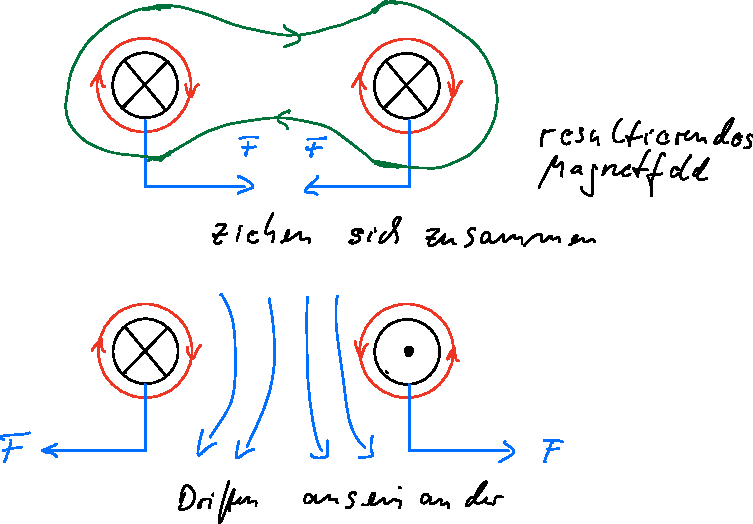
\includegraphics[width=0.6\textwidth]{images/Skizze/05_StromdurchflossenerLeiter_Skizze.pdf}
\caption{Stromdurchflossener Leiter}
%\label{fig:}%% anpassen
\end{figure}

Ist die technische Stromflussrichtung in beiden Seiten gleich, dann
bildet sich ein Magnetfeld um die beiden Leiter herum.

Im Gegensatz dazu ist die technische Stromflussrichtung nicht gleich,
bildet sich das Magnetfeld zwischen den beiden Leitern.

\newpage

\section{Rechte Handregel (Generator
Regel)}\label{rechte-handregel-generator-regel}

\begin{figure}[!ht]% hier: !ht
\centering
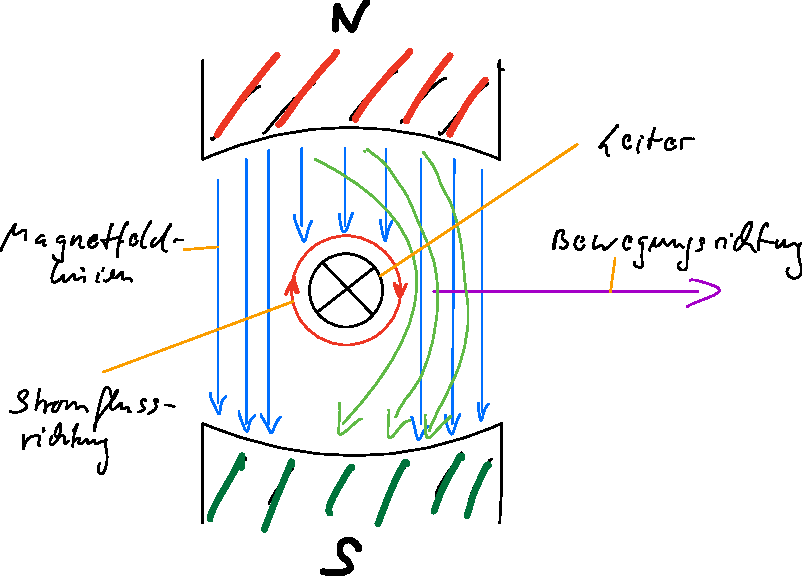
\includegraphics[width=0.6\textwidth]{images/Skizze/01_Generatorregel_Skizze.pdf}
\caption{Generatorregel}
%\label{fig:}%% anpassen
\end{figure}

Wir haben einen Dauermagneten, der Nordpol trifft in die
Innenhandfläche.

Wenn ich bewege, d.~h. die offene Handfläche dreht sich nach rechts,
fließt der Strom Richtung Fingerspitzen.

\section{Linke Handregel (Motor
Regel)}\label{linke-handregel-motor-regel}

\begin{figure}[!ht]% hier: !ht
\centering
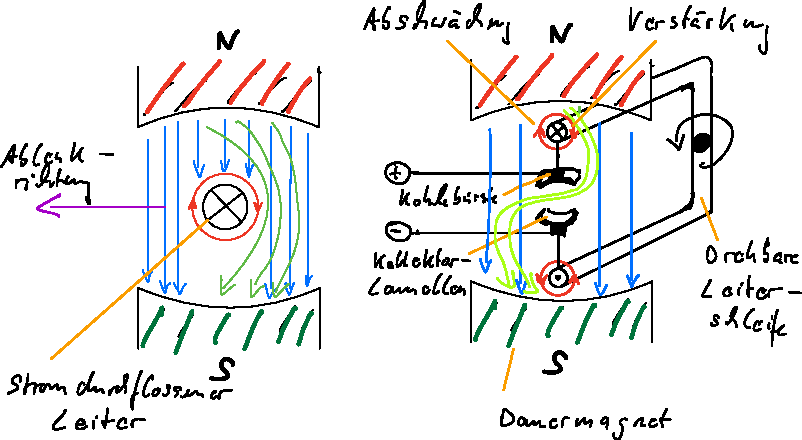
\includegraphics[width=0.6\textwidth]{images/Skizze/02_Motorregel_Skizze.pdf}
\caption{Motorregel}
%\label{fig:}%% anpassen
\end{figure}

Lasse ich Strom fließen, ist die Bewegung nach links.

\section{Das Ohmsche Gesetz}\label{das-ohmsche-gesetz}

Das ohmsche Gesetz zeigt die Beziehung zwischen Spannung, Strom und
Widerstand im Stromkreis. Die Stromstärke steigt mit zunehmender
Spannung und nimmt ab mit zunehmendem Widerstand.

$\boxed{I = \frac{U}{R}} \quad \bigl[\frac{V}{\Omega}\bigl] = A \quad  \boxed{R = \frac{U}{I}} \quad \bigl[\frac{V}{A}\bigl] = \Omega \quad  \boxed{U = R \cdot I} \quad [\Omega \cdot A] = V$

\newpage

\section{Festlegen des Nordpols einer stromdurchflossenen
Spule}\label{festlegen-des-nordpols-einer-stromdurchflossenen-spule}

\begin{figure}[!ht]% hier: !ht
\centering
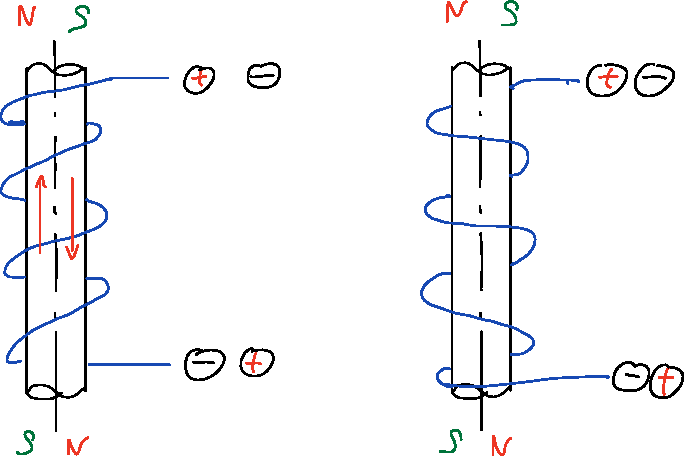
\includegraphics[width=0.6\textwidth]{images/Skizze/03_StromdurchflosseneSpule_Skizze.pdf}
\caption{Stromdurchflossene Spule}
%\label{fig:}%% anpassen
\end{figure}

Wird eine stromdurchflossene Spule mit der rechten Hand so umfasst, dass
die Finger in die technische Stromflussrichtung zeigen, so zeigt der
abgespreizte Daumen in Richtung des Nordpols.

\textbf{Anschluss dahinter} gewickelt, dann zeigt der Daumen nach oben
in Richtung Nordpol.

\textbf{Anschluss davor} gewickelt, dann zeigt der Daumen nach unten in
Richtung Nordpol.

\section{Einsatz von Widerständen}\label{einsatz-von-widerstaenden}

Spannung und Stromfluss zu begrenzen und dadurch Bauteile zu schützen.

Abhängig von Reihen-, Parallel- oder gemischte Schaltung.

\textbf{Anwendung Reihenschaltung}

\begin{enumerate}
\def\labelenumi{(\arabic{enumi})}
\item
  Strombegrenzung
\item
  Spannungsteilung
\end{enumerate}

\textbf{Anwendung Parallelschaltung}

\begin{enumerate}
\def\labelenumi{(\arabic{enumi})}
\item
  Stromflusserhöhung
\item
  Leistungsteilung $\boxed{R_{ges} = \frac{R_{Teil}}{n}}$
\end{enumerate}

\section{Zusammenhang zwischen Stromdichte und
Leitungsquerschnitt}\label{zusammenhang-zwischen-stromdichte-und-leitungsquerschnitt}

Je größer die Fläche, desto kleiner die Stromdichte.

Kleine Fläche, große Stromdichte.

\begin{figure}[!ht]% hier: !ht
\centering
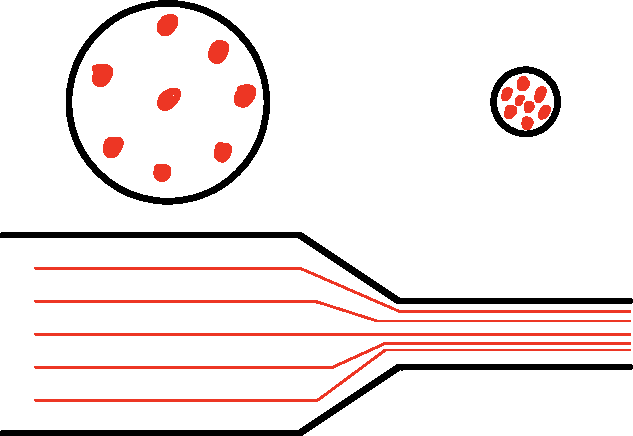
\includegraphics[width=0.4\textwidth]{images/Skizze/04_Stromdichte_Skizze.pdf}
\caption{Stromdichte}
%\label{fig:}%% anpassen
\end{figure}

$\boxed{J = \frac{I}{A}} \quad \bigl[\frac{A}{mm^2}\bigl]$

$\boxed{A = \frac{\rho \cdot l \cdot I}{U_v}} \quad \bigl[\frac{\Omega \cdot mm^2 \cdot m}{m \cdot \Omega}\bigl] = mm^2$
(Mindestquerschnitt, Nennquerschnitt)

$\quad \rho_{Cu} = 0,0178~\frac{\Omega \cdot mm^2}{m}$

\section{Leiterwiderstand}\label{leiterwiderstand}

Leiterwiderstand ist abhängig von der Leiterlänge, Leiterwerkstoff und
von der Leiterfläche.

Guter Leiter -- ist das Material leitend vs.~nicht leitend.

$\boxed{R_l = \frac{\rho \cdot l}{A}} \quad \bigl[\frac{\Omega \cdot mm^2 \cdot m}{m \cdot mm^2}\bigl] = \Omega \quad \rho_{Cu} = 0,0178~\frac{\Omega \cdot mm^2}{m}$

$\boxed{\text{max. Leiterwiderstand} = 1~\Omega}$

\newpage

\section{Reihenschaltung von
Widerständen}\label{reihenschaltung-von-widerstaenden}

\begin{figure}[!ht]% hier: !ht
\centering
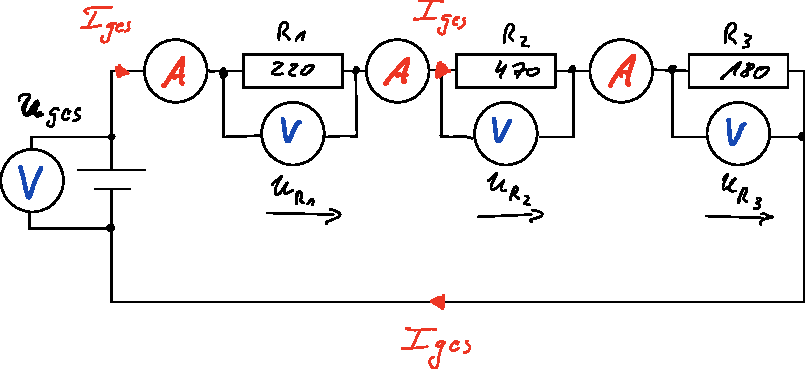
\includegraphics[width=0.6\textwidth]{images/Skizze/07_Reihenschaltung_Widerstaende_Skizze.pdf}
\caption{Reihenschaltung - Widerstände}
%\label{fig:}%% anpassen
\end{figure}

Spannungsteilerschaltung, an den einzelnen Widerständen fällt
individuell eine Spannung ab. Alle Einzelspannungen zusammen addiert
ergibt die Gesamtspannung.

Der Strom bleibt konstant.

\newpage

\section{Innenwiderstand von
Spannungsquellen}\label{innenwiderstand-von-spannungsquellen}

\begin{figure}[!ht]% hier: !ht
\centering
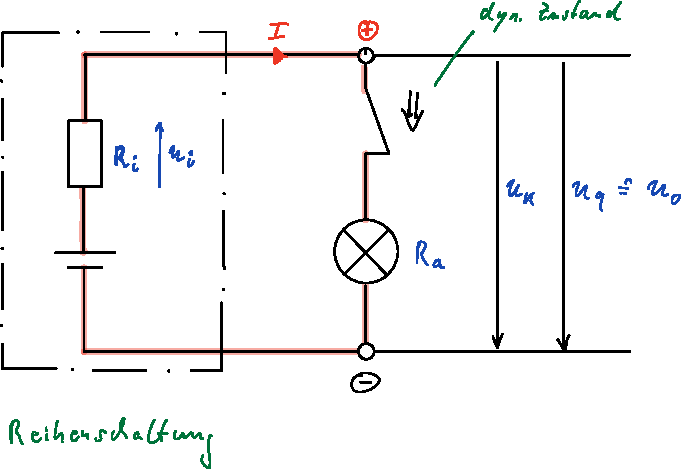
\includegraphics[width=0.6\textwidth]{images/Skizze/14_ Innenwiderstand_von_Spannungsquellen_Skizze.pdf}
\caption{Innenwiderstand von Spannungsquellen}
%\label{fig:}%% anpassen
\end{figure}

\begin{table}[!ht]% hier: !ht 
\centering 
	\caption{}% \label{tab:}%% anpassen 
\begin{tabular}{@{}lll@{}}
\hline
\textbf{Bezeichnung} & \textbf{Benennung} & \textbf{Einheit} \\
\hline
$U_q$ & Quellspannung & $[V]$ \\
$U_0 (U_{Null})$ & Leerlaufspannung & $[V]$ \\
$U_k$ & Klemmenspannung (Last, mit Verbraucher) & $[V]$ \\
$U_i$ & Spannungsabfall am Innenwiderstand & $[V]$ \\
$R_i$ & Innenwiderstand & $[\Omega]$ \\
$R_a$ & Außenwiderstand & $[\Omega]$ \\
$I$ & Stromfluss, -stärke & $[A]$ \\
\hline
\end{tabular} 
\end{table}

Ist der Gesamtwiderstand aller Zellen, ist auch Temperaturabhängig.

Die Klemmenspannung unter Last ist um Spannungsfall niedriger als die
Leerlaufspannung.

$\boxed{U_k = U_q - I \cdot R_i} \quad [V - A \cdot \Omega \to V - V] = V$

$\boxed{R_i = \frac{U_i}{I}} \quad \boxed{U_k = U_q - U_i - U_v} \quad \boxed{R_{ges} = R_i + R_l + R_\text{ü} + R_{La}}$

\newpage

\section{Relais}\label{relais}

Mit einem kleinen Steuerstrom kann ich einen hohen Laststrom schalten.

Wird unterschieden zwischen Schließer-, Öffner- und Wechselrelais.

\begin{figure}[!ht]% hier: !ht
\centering
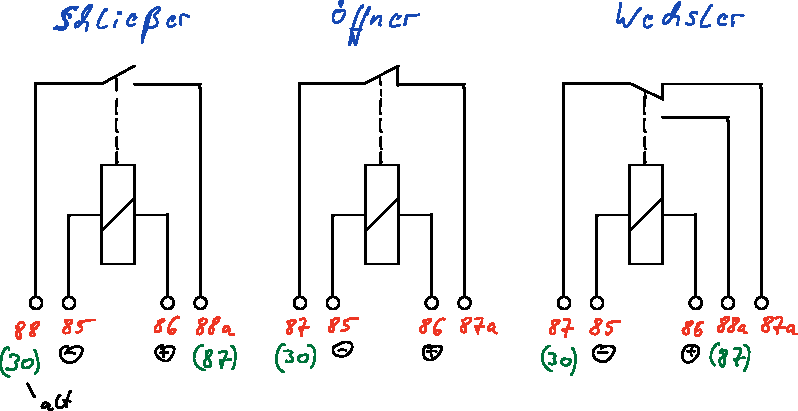
\includegraphics[width=0.7\textwidth]{images/Skizze/08_Relais_Skizze.pdf}
\caption{Relais}
%\label{fig:}%% anpassen
\end{figure}

\textbf{Ströme einer Relaisschaltung}

\begin{figure}[!ht]% hier: !ht
\centering
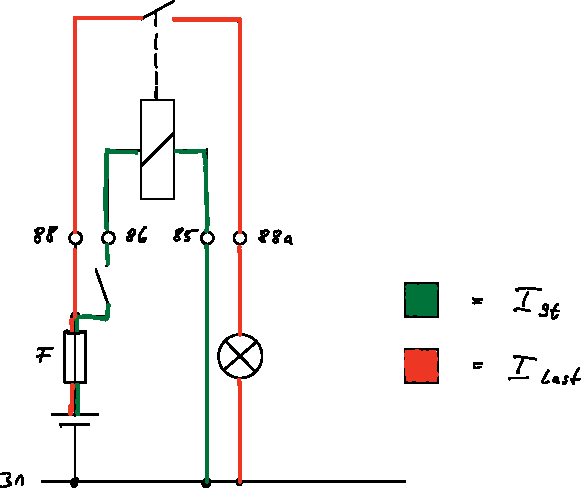
\includegraphics[width=0.4\textwidth]{images/Skizze/09_Stroeme_einer_Relaisschaltung_Skizze.pdf}
\caption{Ströme einer Relaisschaltung}
%\label{fig:}%% anpassen
\end{figure}

\begin{itemize}
\item
  \emph{Steuerstrom:} $50 - 200~mA$
\item
  \emph{Laststrom:} nach Verbraucher und Hersteller
\item
  \emph{Relaisspulenwiderstand:} $50 - 100~\Omega$ (ohne
  Schutzbeschaltung)
\end{itemize}

\newpage

\section{Parallelschaltung von
Widerständen}\label{parallelschaltung-von-widerstaenden}

\begin{figure}[!ht]% hier: !ht
\centering
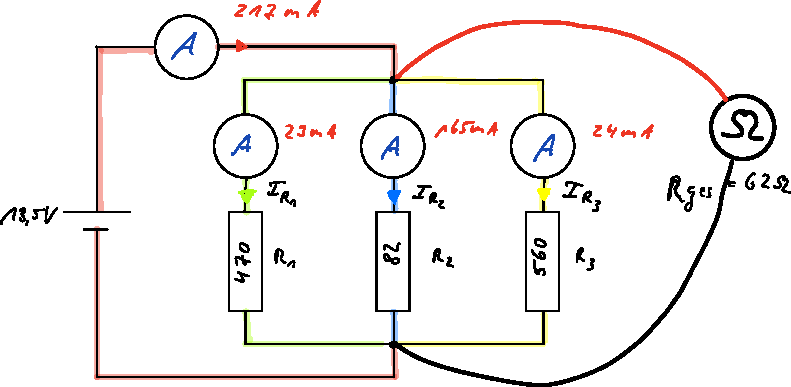
\includegraphics[width=0.6\textwidth]{images/Skizze/19_Parallelschaltung_Widerstaende_Skizze.pdf}
\caption{Parallelschaltung von Widerstände}
%\label{fig:}%% anpassen
\end{figure}

Stromteilerschaltung, der abfallende Einzelstrom ergibt, addiert den
Gesamtstrom.

Der Gesamtwiderstand der Schaltung ist immer kleiner als der kleinste
Einzelwiderstand.

Spannung ist überall gleich.

Ersatzwiderstand

$\boxed{R_{ges} = \frac{R_{Teil}}{n}}$

n = Anzahl der Widerstände (gleich große Widerstände)

$\boxed{R_{ges} = \frac{R_1 \cdot R_2}{R_1 + R_2}} \quad R_{ges} = \frac{1}{\frac{1}{R_1} + \frac{1}{R_2} + \frac{1}{R_3}}$

$\to R_{1} = \frac{1}{\frac{1}{R_{ges}} - \frac{1}{R_2} - \frac{1}{R_3}} \quad \to R_{2} = \frac{1}{\frac{1}{R_{ges}} - \frac{1}{R_1} - \frac{1}{R_3}} \quad \to R_{3} = \frac{1}{\frac{1}{R_{ges}} - \frac{1}{R_1} - \frac{1}{R_2}}$

\section{Leistung}\label{leistung}

Leistung ist das Produkt aus Spannung und Strom.

Mit 1 Volt Spannung und 1 Ampere Strom haben wir 1 Watt Leistung.

$\boxed{P = U \cdot I} \quad [V \cdot A] = W \quad \boxed{P = \frac{U^2}{R}} \quad \boxed{P = R \cdot I^2}$

\textbf{Lampe} $12~V/55~W$

$R_{La} = \frac{U^2}{P} \quad I_{tat} = \frac{U_k}{R_{La}} = \frac{U_{ges} - U_v}{R_{La}} \quad P_{tat} = U_k \cdot I_{tat}$

\newpage

\section{Spannungsverlust,
Spannungsfall}\label{spannungsverlust-spannungsfall}

Nennquerschnitt Tabellenbuch (\textcite{bell:2021:tabellenbuchKfz} S. 280)

Klemmbezeichnung Tabellenbuch (\textcite{bell:2021:tabellenbuchKfz} S. 273)

Spannungsfall Tabellenbuch (\textcite{bell:2021:tabellenbuchKfz} S. 280)

\begin{figure}[!ht]% hier: !ht
\centering
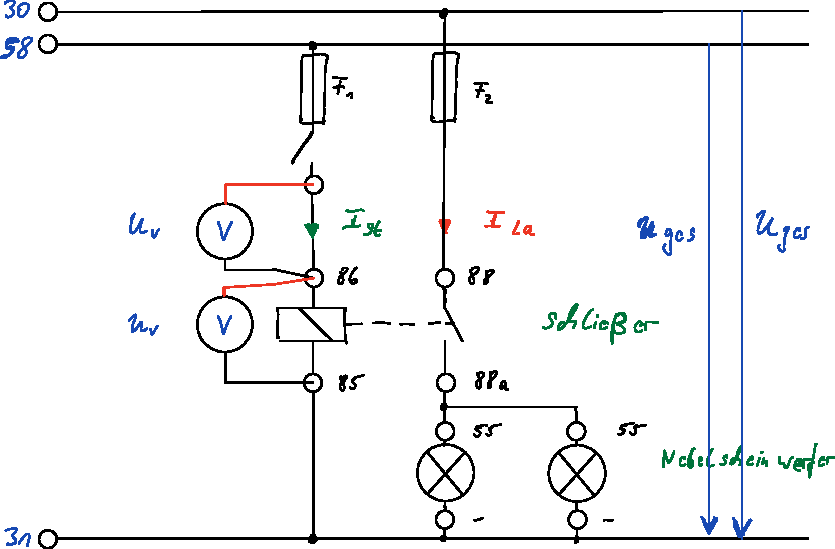
\includegraphics[width=0.65\textwidth]{images/Skizze/13_Spannungsverlust_Skizze.pdf}
\caption{Spannungsverlust}
%\label{fig:}%% anpassen
\end{figure}

\begin{table}[!ht]% hier: !ht 
\centering 
	\caption{}% \label{tab:}%% anpassen 
\begin{tabular}{@{}lll@{}}
\hline
\textbf{Bezeichnung} & \textbf{Benennung} & \textbf{Einheit} \\
\hline
$U_{ges}$ & Gesamtspannung & $[V]$ \\
$U_v$ & Spannungsverlust & $[V]$ \\
$U_k$ & Klemmspannung & $[V]$ \\
$R_l$ & Leiterwiderstand & $[\Omega]$ \\
$I$ & Stromfluss, Stromstärke & $[A]$ \\
\hline
\end{tabular} 
\end{table}

Spannungsverlust in einem stromdurchflossenen Leiter entsteht in Folge
des Leiterwiderstandes, der sich am Verbraucher als Verlust auswirkt.

$U_{ges} = U_v + U_k \quad U_v = R_l \cdot I \quad U_k = U_{ges} - R_l \cdot I$

$\boxed{U_v = \frac{\rho \cdot l \cdot I}{A}} \quad \bigl[\frac{\Omega \cdot mm^2 \cdot m \cdot A}{m \cdot mm^2}\bigl] = V \quad \rho_{Cu} = 0,0178~\frac{\Omega \cdot mm^2}{m} \quad \boxed{U_{v_{max}} = 0,5~V}$

\newpage

\section{Potenzialbestimmung}\label{potenzialbestimmung}

\begin{figure}[!ht]% hier: !ht
\centering
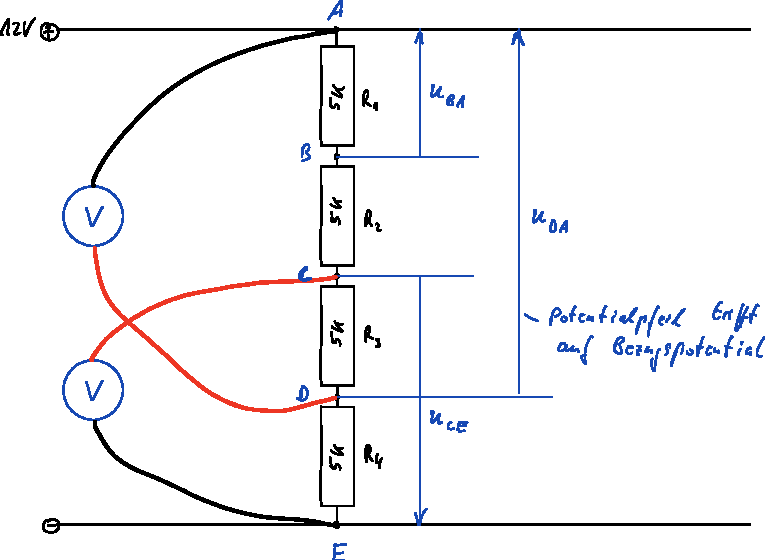
\includegraphics[width=0.6\textwidth]{images/Skizze/28_FT_Potentialbestimmung.pdf}
\caption{Potentialbestimmung}
%\label{fig:}%% anpassen
\end{figure}

Klemmenspannung und Potential

\begin{itemize}
\item
  $U_{R_1} = 3~V$, $U_{R_3} = 3~V$
\item
  $U_{CE} = 6~V$, $U_{BA} = -3~V$, $U_{DA} = -9~V$
\end{itemize}

Möchte man das/ein Potential an einem Punkt in einem Stromkreis
messen/bestimmen, bezieht man sich immer auf ein Bezugspotenzial. Die
Schreibweise dieser Messung lautet dann zum Beispiel $U_{CE}$, hierbei
möchte ich also das Potential C messen, C ist der erste Buchstabe, an
ihm wird der \emph{rote Clip} des Multimeters angeschlossen. Das
Bezugspotenzial hierbei E ist der zweite Buchstabe, hier wird
grundsätzlich der \emph{schwarze Clip} des Multimeters angeschlossen.
Potentialbestimmungen können auch zeichnerisch dargestellt werden.
Hierbei lautet die Vereinbarung, die Pfeilspitze des Spannungs- oder
Potentialpfeils trifft immer auf das Bezugspotenzial. Beispiel
$U_{DA}$.

\newpage

\section{Brückenschaltung -
Brückenspannung}\label{brueckenschaltung-brueckenspannung}

\begin{figure}[!ht]% hier: !ht
\centering
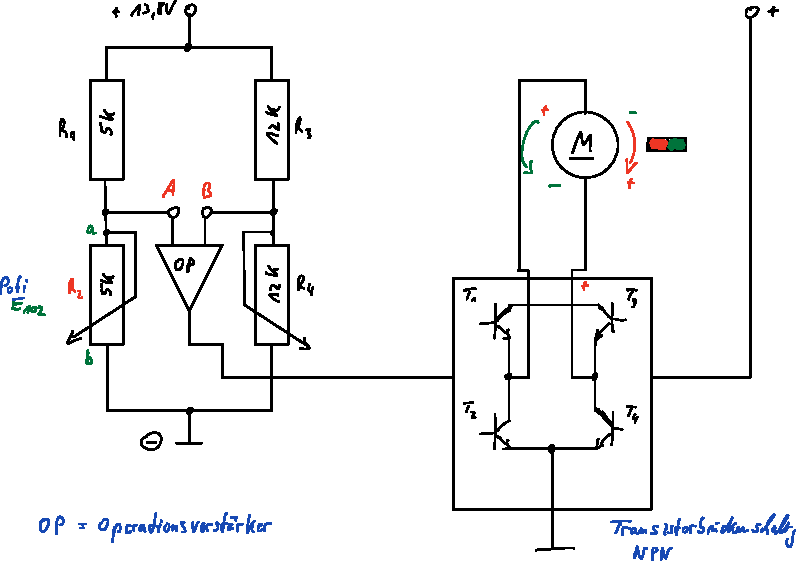
\includegraphics[width=0.6\textwidth]{images/Skizze/28_FT_Brueckenschaltung.pdf}
\caption{Brückenschaltung}
%\label{fig:}%% anpassen
\end{figure}

$U_{A\text{-}} = 6,9~V$, $U_{B\text{-}} = 6,9~V$, $U_{AB} = 0~V$
(keine Differenz)

$U_{A\text{+}} = -6,9~V$, $U_{B\text{+}} = -6,9~V$, $U_{AB} = 0~V$
(keine Differenz)

Poti $\to R_2 = 1~k$

$I_{Li} = \frac{U_{ges}}{R_{{Li}_{ges}}} = \frac{U_{ges}}{R_1 + R_2} = \frac{13,8}{5000 + 1000} =0,0023~A$

$U_{R_1} = R_1 \cdot I_{Li} = 5000~\Omega \cdot 0,0023~A = 11,5~V$

$U_{A\text{+}} = -11,5~V$, $U_{B\text{+}} = -6,9~V$,
$U_{AB} = -4,6~V$

$I_{Re} = \frac{U_{R_3}}{R_3} = \frac{11,5}{12000} =0,00096~A$

$R_4 = \frac{U_{R_4}}{I_{Re}} = \frac{U_{ges} - U_{R_3}}{I_{Re}} = \frac{13,8 - 11,5}{0,00096} = 2395,83~\Omega$
